\documentclass[oneside]{memoir}
\usepackage[]{tikz}
\usetikzlibrary{shapes,arrows,chains}
\usetikzlibrary[calc]
\usepackage{amsmath}
\usepackage[]{graphicx}

\usepackage{csquotes}


  
\setulmarginsandblock{1.5cm}{1.5cm}{*}
\setlrmarginsandblock{4cm}{1.5cm}{*}
\checkandfixthelayout

\renewcommand{\thesection}{}
\newcommand{\yhat}{\ensuremath{\hat{\vec{y}}}}
\title{Neural Networks \\ \small{A simple example}}
\author{Henrik Lund Mortensen}

\begin{document}

\maketitle


\section{Neural network as a classifier}
The neural network (NN) presented in this note solves a classification problem; Given $\vec{x}$ and a set of classes $Y$, determine which class $\vec{x}$ belongs to. 

The NN is a nonlinear function with a lot of parameters, or weights $\{W,b\}$.

\begin{equation}
  \label{NN}
\yhat{} = f_{NN}(\vec{x},W,b)
\end{equation}

The output is a vector, $\hat{\vec{y}}$, where the $i$'th entry is the estimated probability that the input belongs to the class $\vec{y}_{k} = \delta_{ik} \in Y$. The training consists of finding the weigths such that $\yhat{}$. 


% \begin{tikzpicture}
%   \node at (0,1) {Hello!};
%   \node at (13,1) {Hello!};

%   \node at (0.1)

%   \node at (0,10) {Hello!};
%   \node at (13,10) {Hello!};



% \end{tikzpicture}
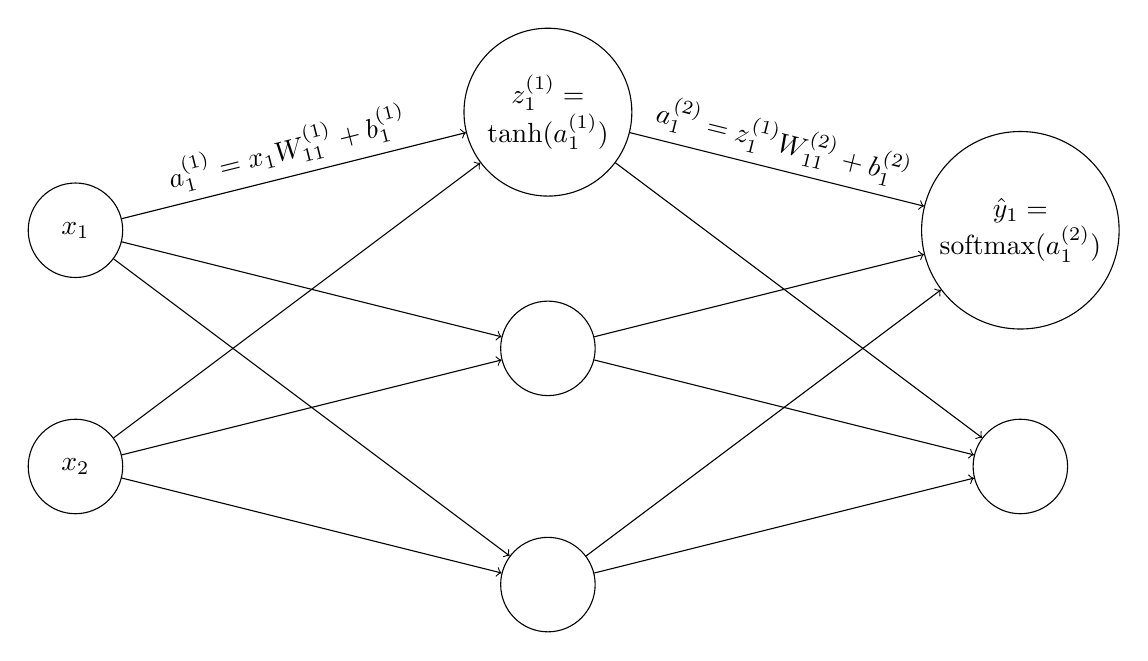
\begin{tikzpicture}
\centering
\node at (0,0) {  };
\node at (0,6.66667) {  };
\node at (12,6.66667) {  };
\node at (12,0) {  };
\node[draw,circle,minimum size=1.2cm,name=n00,align=center] at (0,1.83333) {$x_2$};
\node[draw,circle,minimum size=1.2cm,name=n01,align=center] at (0,4.83333) {$x_1$};
\node[draw,circle,minimum size=1.2cm,name=n10] at (6,0.333333) {};
\node[draw,circle,minimum size=1.2cm,name=n11] at (6,3.33333) {};
\node[draw,circle,minimum size=1.2cm,name=n12,align=center] at (6,6.33333) {$z_{1}^{(1)} =$\\$ \text{tanh}(a_{1}^{(1)})$};
\node[draw,circle,minimum size=1.2cm,name=n20] at (12,1.83333) {};
\node[draw,circle,minimum size=1.2cm,name=n21,align=center] at (12,4.83333) {$\hat{y}_{1} =$\\$ \text{softmax}(a_{1}^{(2)})$};
\draw[->,name=a0010] (n00) -- (n10);
\draw[->,name=a0011] (n00) -- (n11);
\draw[->,name=a0012] (n00) -- (n12);
\draw[->,name=a0110] (n01) -- (n10);
\draw[->,name=a0111] (n01) -- (n11);
\draw[->,name=a0112] (n01) -- node[sloped,anchor=center,above] {$a_{1}^{(1)} =x_{1}W_{11}^{(1)} + b_1^{(1)}$} (n12);
\draw[->,name=a1020] (n10) -- (n20);
\draw[->,name=a1021] (n10) -- (n21);
\draw[->,name=a1120] (n11) -- (n20);
\draw[->,name=a1121] (n11) -- (n21);
\draw[->,name=a1220] (n12) -- (n20);
\draw[->,name=a1221] (n12) -- node[sloped,anchor=center,above] {$a_{1}^{(2)} =z_{1}^{(1)}W_{11}^{(2)} + b_1^{(2)}$} (n21);
\end{tikzpicture}


% \footnote{The are often issues of overfitting, where the training data }

% By adjusting the weights, the NN will (hopefully) be able to determine which class an input vector belongs to. 
% The NN is trained on a set of training examples, $\{\vec{x},\vec{y}\}$, where $\vec{y} \in Y$, by adjusting the weights, $\{W,b\}$.

\begin{equation}
  \label{activation function tanh}
\text{Activation function} = \tanh(\vec{x})
\end{equation}

\begin{equation}
  \label{softmax}
  \text{softmax}(\vec{x})_i = \frac{e^{\vec{x}_i}}{\sum_k e^{\vec{x}_k}}
\end{equation}
\begin{equation}
  \label{cross entropy}
  \text{Err}(\hat{\vec{y}},\vec{y}) = \frac{-1}{N} \sum_{n\in N} \sum_{i \in C} \vec{y}_{n,i} \log \hat{\vec{y}}_{n,i}
\end{equation}

\section{Backpropagation} 
The weigths are updated by calculating the gradient of the loss function w.r.t. the individual weigths. These gradients can be efficiently calculated by using the backpropagation algorithm.

At the heart of the backpropagation algorithm is the chain rule,
\begin{equation}
  \label{chain rule}
  \frac{\partial x}{\partial y} = \frac{\partial y}{\partial z} \frac{\partial z}{\partial x}.
\end{equation}




\subsection{Local gradients}

\begin{equation}
  \label{dLdyhat}
  \frac{\partial L}{\partial \hat{\vec{y}}_i} = \frac{-1}{N} \frac{\vec{y}_i}{\hat{\vec{y}}_i}
\end{equation}
\begin{equation}
  \label{dyhatda}
  \frac{\partial \hat{\vec{y}}_i}{\partial \vec{a}_j^{(N_{\text{layer}})}} = \hat{\vec{y}}_i ( \delta_{ij} - \hat{\vec{y}}_i)
\end{equation}
so that (assuming $\vec{y}_i= \delta_{is}$ for some $s$) 
\begin{equation}
  \label{dLdyhat times dyhatda}
  \frac{\partial L}{\partial \hat{\vec{y}}} \cdot \frac{\partial \hat{\vec{y}}}{\partial \vec{a}^{(N_{\text{layer}})}}  = \frac{\yhat- \vec{y}}{N}
\end{equation}

\begin{equation}
  \label{dadW}
  \frac{\partial \vec{a}_i^{(p)}}{\partial W^{(p)}_{jk}} = 
  \begin{cases}
    \delta_{ik} \vec{z}_j^{(p-1)} & \text{if} p > 1 \\
    \delta_{ik} \vec{x}_j& \text{if} p = 1 \\
  \end{cases}
\end{equation}
\begin{equation}
  \label{dadb}
  \frac{\partial \vec{a}_i^{(p)}}{\partial b^{(p)}_{j}} = \delta_{ij}
\end{equation}
\begin{equation}
  \label{dadz}
  \frac{\partial \vec{a}_i^{(p)}}{\partial \vec{z}^{(p-1)}_{j}} = W_{j,i}^{(p)}
\end{equation}



The recursive formula for calculating the gradient of all weights and biases is given by
\begin{align}
  \label{dLdb_i}
  \frac{\partial L}{\partial \vec{b}^{(i)}} &= \frac{\partial L}{\partial \vec{b}^{(i+1)}} \cdot{W}^{T(i+1)} \circ (1-\vec{z^{(i)}}\circ \vec{z^{(i)}})\\
  \frac{\partial L}{\partial \vec{b}^{(N_\text{layer})}} &= \frac{\hat{\vec{y}}-\vec{y} }{N_{\text{samples}}}\\
  \label{dLdW_i}
  \frac{\partial L}{\partial \vec{W}^{(i)}} &=
                                              \begin{cases}
                                                \vec{z}^{(i-1)} \otimes \frac{dL}{db^{(i)}} & \text{if } i \geq 2 \\
                                                \vec{x}\otimes \frac{dL}{db^{(i)}}  & \text{if } i = 1
                                              \end{cases}
\end{align}



\begin{figure}
  \centering
  \includegraphics[scale=0.8]{decisionBoundary.png}
\end{figure}

\end{document}